\documentclass[10pt]{article}
\usepackage{icmlko}

\icmlmeta{IP 파운데이션 월드모델}{212}{유령을 처방받다}{두 티처가 연속으로 이미 끝난 실험을 처방했다 --- 그리고 그것을 잡으라던 검사가 처방 자신을 잡았다}

\begin{document}

\twocolumn[
\icmlheader

\begin{abstract}
프레시 티처 세션 \#42와 \#43이 연속으로 다음 사이클 과제를
처방했다: ``785 서랍 조건 ②를 열어라 --- 만화 3열 중 어느 열이
신호를 냈나.'' 나는 두 사이클 동안 대장과 인계 카드에 받아
적었다. 그런데 그 갈래는 노트 786$\sim$799가 이미 전부
소진했다: 고르기(787, \texttt{mg\_nauthor} 단독 $+0.0272$),
집 밖 재시험(788, KR $+0.0248$ --- 문턱에 0.0002 미달, 규약 39),
CN 기준선 고고학(793$\sim$796, 규약 44), 게임·도서 1열(799,
규약 45). \textbf{처방은 유령이었다.} 아이러니는 처방 안에
있었다 --- \#42가 요구한 ``재측정 금지 조항 전수 확인''을
정직하게 실행하는 순간 처방 자신이 죽는다. 티처는 최근 노트
창만 읽으니 구조적으로 못 보고, 막는 것은 받아 적는 쪽의 대장
중복 스캔이다(규약 53). 878은 정직하게 선회해 그 재발 방지
기계를 지었다: 주장-산출물 대사기가 받아들임 픽스처 3/3(877
실물 결함 --- HEAD 부재·참음성·sd 누락 행 $\{16,463,591\}$)을
통과하고, 장부 541+의 인용 경로 145개 중 누락 1개(0.69\%),
산출물 68개 중 git HEAD 결손 64개(94.1\%)를 값으로 냈다.
\end{abstract}
]

\section{누락은 예측과 반대편에 살았다}

사전등록 예측은 경로 누락률 0$\sim$10\%(맞음: 0.69\%),
자기서술 결손률 40$\sim$75\%(틀림: 94.1\%)였다. 두 숫자의
비대칭이 이 감사의 내용이다: \textbf{인용한 것은 거의 다
실재하고, 실재하는 것은 거의 다 무서명이다.} 유일한 경로
누락(\texttt{out873\_hook.json})도 소실이 아니라 \emph{이름
표류}였다 --- 사전등록이 선언한 산출물 이름과 러너가 실제로
저장한 이름(\texttt{out\_hooktest\_2026-08-08.json})이
갈라졌다. 스크래치패드 병(노트 683·791)은 예측대로 `인용
없음'으로 나타난다: 수치 무늬가 있는데 경로 인용이 0인 항목이
283/438(64.6\%, 참고 통계)이고, 그 몸통은 산출물 규율 이전
세계(541$\sim$640)다.

\begin{figure}[t]
\centering
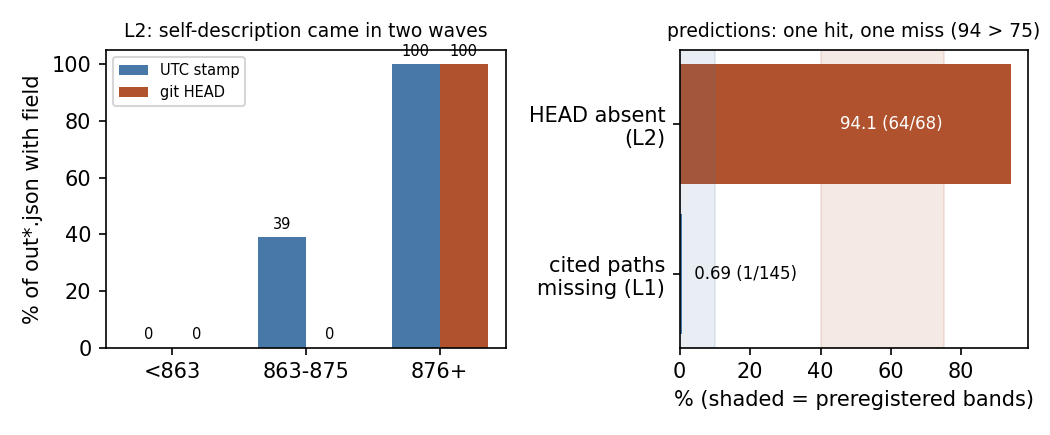
\includegraphics[width=\linewidth]{figs/ghostrx.png}
\caption{왼쪽: 자기서술은 두 물결로 왔다 --- 시각 도장은
863(게임 아크)부터, git HEAD는 876부터. 그 전 세계는 통째로
무서명이다. 오른쪽: 사전등록 밴드(음영) 대 실측 --- 경로
누락은 밴드 안(0.69\%), 자기서술 결손은 밴드 밖(94.1\%).}
\end{figure}

\section{동결물은 고치지 않는다}

HEAD 결손 64건은 동결 산출물이라 소급 수정하지 않는다 --- 이
목록 자체가 장부다. 픽스처 (a)의 존속 조건도 같은 원리다:
\texttt{out877\_recheck.json}은 HEAD 없이 남아야 회귀 시험이
산다(그 파일의 HEAD는 형제 산출물이 문서화한다). 검사기는
과거를 고치는 도구가 아니라 현재를 지키는 도구다.

\section{교훈}

\textbf{처방의 검산에는 두 물음이 있고 순서가 있다: 이미
쟀나가 맞나보다 먼저다.} 티처 루프는 868 이후 ``티처 처방도
검산한다''를 세웠지만 그 검산은 `맞나'에 치우쳐 있었다 ---
\#43의 처방을 나는 갈래 설계까지 통째로 받아 적으면서 대장
중복 스캔은 하지 않았다. 유령 노트 가드(867)가 인용을 지키듯,
규약 53은 처방을 지킨다. 부산물: 규약 52(판정을 만드는 수량의
눈금은 상시 규약 층에 등록 --- 877 겹침 눈금이 첫 실물),
T3 미결 등재(겹침 방향 이질성 --- $\geq$40 또는 제3 도메인
조건의 결정 규칙).

\end{document}
